\pagebreak
\subsection{Launch Campaign}
\subsubsection{Flight preparation activities during launch campaign} %.... maybe some of this is currently in chapter 6
The scientific and pneumatic flight preparations can be found in Section \ref{prep_for_Esrange}.

On the first day of the campaign the experiment boxes were mounted into the gondola for the first time to check where the gondola fixation points should be. Once this was checked the box was dismounted again for final preparations. Styrofoam was fixed onto the bottom of the gondola to act as extra support for the boxes. It was fixed with the same double sided tape as was used to fix the Styrofoam to the walls of the experiment boxes.

Once the CAC box was fully integrated with the AirCore it was discovered that one temperature sensor required re soldering. 

During preparations for the E-link test it was discovered that the The Amphenol RJF21B connector was built in the incorrect configuration and it had to be dismantled and rebuilt before E-link testing could be completed.

During the Flight Compatibility Test (FCT) it was discovered that the experiment was sensitive to the Radio Frequencies (RF) emitted from the VHF radios used. If the VHF radios were used within a 10-15m radius of the experiment box errors would appear in the sensor data. In the most extreme case this caused a complete failure of the software and no more data was received until a power cycle was completed. Following this discovery a radio silence area was set around the experiment to prevent these errors from occurring again. It is thought that this phenomenon was caused by two factors, the first being that the boxes housing the experiment have very large surface areas which are completed covered in aluminum and are grounding the electronics. Therefore when the experiment was on if RF interfered with the floating ground point in the boxes surface this can affect the grounding voltage. The second factor was the fact that the I2C connection was spread across very long wires making them more susceptible to interference. This also gave some background to the sensor issues experienced during thermal testing.

Just before mounting the box onto the gondola for the final time all sides of the box were taped with kapton tap to cover any small gaps in between the walls and the structural bars.

\subsubsection{Flight performance}
The flight began nominally with data being down linked as expected. There were some communication losses before takeoff but these were to be expected from the gondola antenna being too close to the ground.

Thermal systems were observed from the ground station to be operating nominally.

After takeoff the software successfully entered ascent mode and the CAC successfully opened. Thermal control continued nominally.

At the first sampling point for the AAC subsystem the software operated as it should attempting to turn on the pump however the pump failed to switch on and caused a full reset of the board. After the board reset the software could correctly re-identify the mode and reopen the CAC valve. However manual control was taken in an attempt the remedy the pump. Unfortunately all attempts to start the pump were unsuccessful during ascent and float phases.

During the descent phase in order to preserve the samples in the CAC no further attempts were made to start the pump as if the CAC valve closed and reopened it would compromise the samples within it.

From takeoff until the landing there were no sensor errors as had been observed during testing. It is thought that the sensor errors during testing may have been due to RF from mobile phones and other on ground emitters. This would explain why there were errors on ground but not during flight.

Upon recovery it was noted that all mechanical systems operated nominally.

\subsubsection{Recovery}
The recovery checklist, in Section \ref{sec:recovery-checklist}, was given to the recovery team to collect the CAC. Due to low cloud cover it was not possible to make a recovery by helicopter. Instead the recovery team drove out to the landing site before hiking through several kilometers of forest. They found the gondola had landed onto the air inlet and outlet tubes however no damage was observed. It is thought that the gondola came down slowly due to the trees and tilted at the last moment. Dirt and forest debris was inside all three tubes. 

The CAC was then returned to Esrange at around 1am the same night. It was immediately hooked up to the analyzers which were previously prepared.

Tne AAC returned the following night at around 2am and was also immediately investigated to see if any samples had been collected.

Both systems were returned before the gases inside the tubes and bags would have been too mixed. The TUBULAR Team is very grateful to all who made this recovery happen so fast given the conditions.

\subsubsection{Post flight activities} \label{post_flight}

% The CAC was immediately hooked up to the gas analyzer once it was returned. It was clear relatively quickly that samples had been collected and the data continued to go through the analyzer for around 45 minutes. The sampled air was saved in smaller pieces of tubing to allow for potential further analysis at a later date. As this data then needed to go through significant amounts of post processing no further action was taken. 

The CAC system was recovered and brought back to Esrange approximately 13 hours after the gondola landed, and was immediately hooked up to the gas analyzer. For the analysis purposes, parts 10 to 17, shown in Figure \ref{fig:CAC-schematic} were removed. The magnesium perchlorate filter was also removed and wrapped in plastic foil for sealing reasons, and was taken by the FMI people. The fill gas was connected to the quick connector body (9), seen in Figure \ref{fig:CAC-schematic}, and since the CAC valve closed at 6 km of altitude, one would expect a pressure decrease. In that case it would be necessary to fill the coil with fill gas, and bring it to ambient pressure, before connecting it to the analyzer. But no pressure change was seen. This could only mean two things: either there was a leak and ambient air entered the coil or the CAC valve never worked and the fill gas from the flushing procedure was still there. Next, the Picarro analyzer was connected to the quick connector body (1) as seen in Figure \ref{fig:CAC-schematic}. Few moments later, Picarro read the sample and the first readings showed up in the screen, seen in Figure \ref{fig:first-readings} \ref{fig:first-readings}.     

\begin{figure}[H]
    \begin{align*}
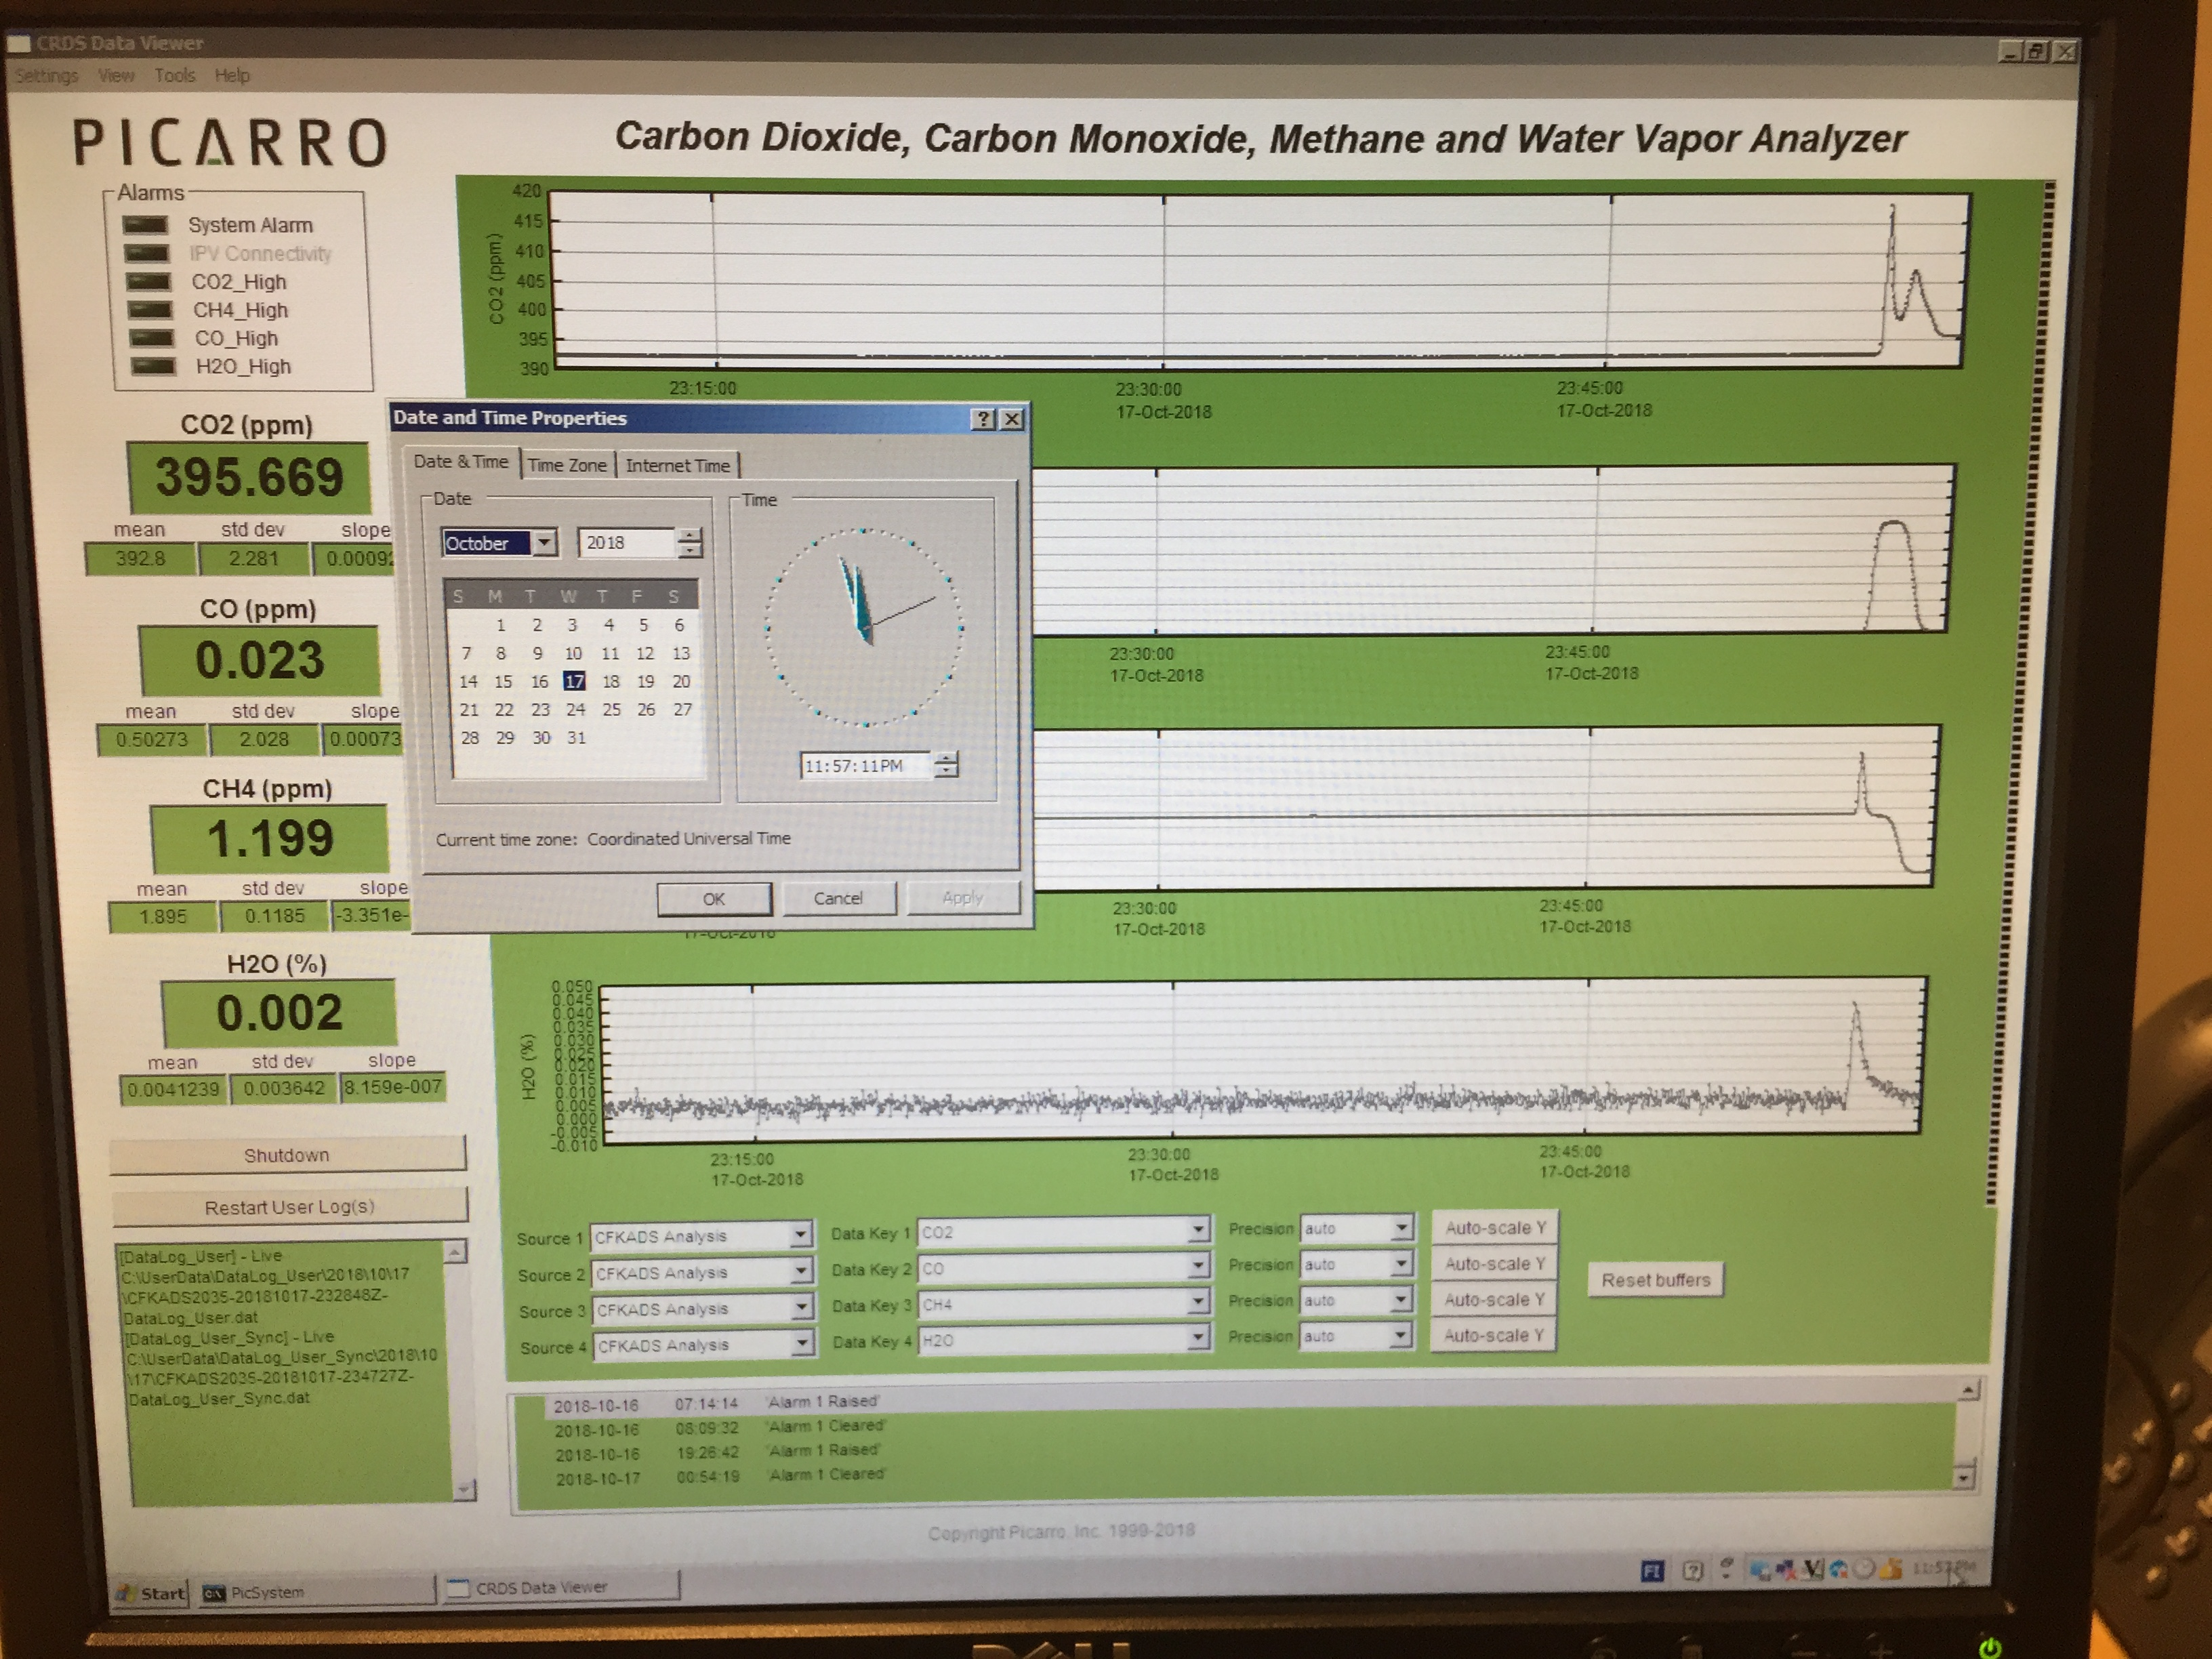
\includegraphics[width=0.9\linewidth]{7-data-analysis-and-results/img/StartofCACanalysis.png}
    \end{align*}
    \caption{First Readings of the CAC. From top to bottom: $CO_2$ ppm, $CO$ ppm, $CH_4$ ppm and cavity pressure. \label{fig:first-readings}}
\end{figure}

As seen in Figure \ref{fig:first-readings} there was a sudden increase in the concentrations and this was the fill gas that had remained, as expected, in the coil. After a while, there was a sudden decrease in the concentrations, and that was the start of the actual sample. The whole CAC profile can be seen in Figure \ref{fig:CAC-profile}   

\begin{figure}[H]
    \begin{align*}
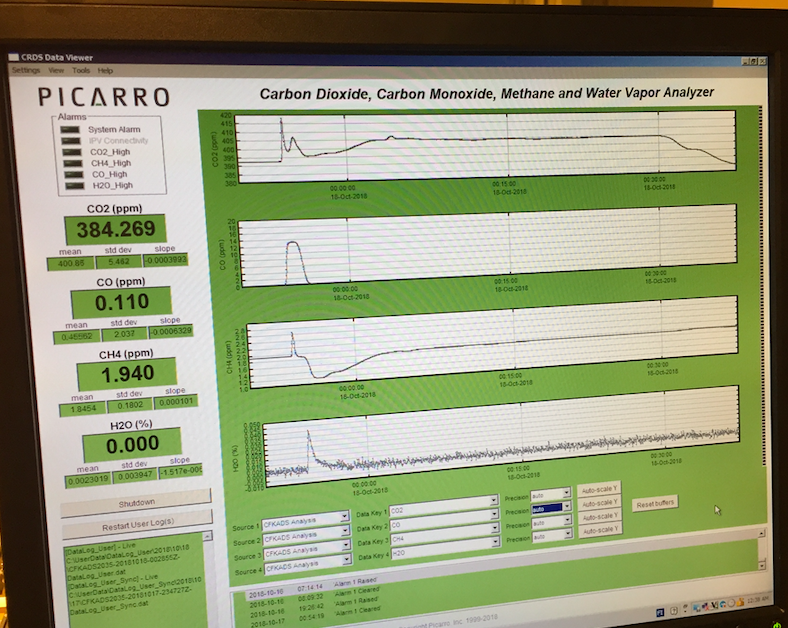
\includegraphics[width=0.9\linewidth]{7-data-analysis-and-results/img/CACprofile.png}
    \end{align*}
    \caption{CAC Complete Profile after the Analysis was Completed. From top to bottom: $CO_2$ ppm, $CO$ ppm, $CH_4$ ppm and cavity pressure. \label{fig:CAC-profile}}
\end{figure}

The slight increase in the $CO_2$ and $CH_4$ concentrations in Figure \ref{fig:CAC-profile} flagged the beginning of the tropospheric part of the sample. After approximately 40 minutes the CAC sample was almost finished and it could be confirmed that the CAC valve was leaking, letting ambient air enter the coil. Even though air from the ground entered the coil, the humidity levels were kept low, because of the magnesium perchlorate filter.  

The CAC system managed to sample the stratosphere and the troposphere down to 6 km of altitude. The lower parts of the profile represent ambient air that went inside the coil through the valve. The analysis of the results can be seen in Section \ref{sec:scientificresults}.

After the analysis was completed, the stratospheric part of the sample was saved into a sampler, composed of fifteen smaller tubes as seen in Figure \ref{fig:aircore-sampler}. This part of the sample, will be further analyzed for isotopes and other atmospheric gases.

For the AAC unfortunately due to the pump failure no data was collected. A post flight failure analysis was carried out on the pump and this can be seen in Section \ref{sec:failureanalysis}.

Data received by the ground station was also analyzed to find the pressure and temperature profiles during the flight. This was completed on MATLAB and was shown during the post flight briefing at campaign.


